\subsubsection{Configuración del cliente LDAP seleccionado}

La configuración del cliente LDAP es crucial para la comunicación efectiva entre la aplicación web y el AD. En esta sección, se detallará el proceso de configuración del cliente LDAP seleccionado, ldapts.

\textbf{Creación de la instancia del cliente}

La creación de la instancia del cliente LDAP (\autoref{fig:ldap-client-initialization}) es un proceso modular que permite incorporar opciones de configuración personalizadas. La función \textbf{getLDAPClient} , la toma las opciones por defecto de la configuración del sistema, definida en el objeto \textbf{config}, y permite la sobrescritura de parámetros mediante el uso de la función \textbf{deepmerge}. De este modo, se asegura flexibilidad en la configuración sin comprometer las configuraciones base.

\begin{figure}[H]
    \centering
    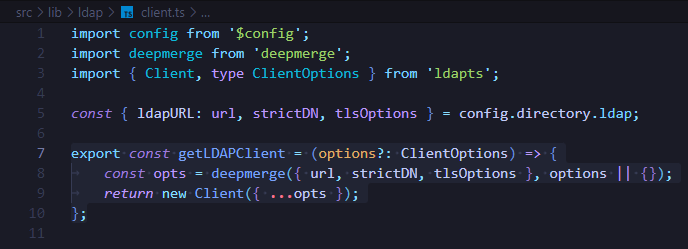
\includegraphics[width=\linewidth]{images/code/ldap-client-initialization.png}
    \caption{Creación del cliente LDAP con ldapts}
    \label{fig:ldap-client-initialization}
\end{figure}

En el fragmento de código de la \autoref{fig:ldap-client-initialization}, se extraen las configuraciones necesarias para la conexión con el AD (como url, strictDN y tlsOptions) y se combinan con las opciones adicionales que se pueden pasar al crear la instancia del cliente LDAP.

\textbf{Manejadores de autenticación}

Para asegurar una operación segura y eficiente del cliente LDAP durante el ciclo de vida de las solicitudes HTTP en la aplicación, se implementaron dos manejadores (handlers) clave en el archivo \textit{src/hooks.server.ts}:
\begin{itemize}
    \item \textbf{authenticationSetHandler}: Este manejador se encarga de inyectar una función de autenticación en las variables locales del evento. Esta función, llamada auth, valida la presencia de un token de acceso y un token de sesión, y si ambos son válidos, realiza la operación bind con el cliente LDAP, utilizando las credenciales del usuario autenticado (\autoref{fig:authentication-set-handler}).
    \item \textbf{ldapUnbindHandler}: Este manejador asegura que el cliente LDAP cierre correctamente la conexión después de procesar cada solicitud, mediante la operación unbind, liberando así los recursos de forma segura y evitando conexiones abiertas innecesarias (\autoref{fig:ldap-unbind-handler}).
\end{itemize}

Este enfoque garantiza que el cliente LDAP esté disponible solo cuando se necesita y que se libere de manera adecuada al final de cada solicitud, lo que mejora tanto la seguridad como el rendimiento general del sistema. Al centralizar la desconexión en un solo lugar, se garantiza que el cliente siempre se cierre adecuadamente después de cada solicitud, evitando conexiones abiertas que podrían saturar el sistema o generar problemas de seguridad. Esta práctica contribuye a una gestión más eficiente y segura del ciclo de vida del cliente LDAP.
